\chapter{Testes empíricos e análise dos resultados}

TEXTO AQUI.

\section{Roteiro e fundamentação do teste proposto}

Este trabalho propõe como teste de validação para técnica de classificação
descrita nos capítulos anteriores um esquema simples de comparação de
expectativas, haverá um grupo de imagens previamente classificado por agentes
humanos, e outra classificação, para este mesmo grupo de imagens, gerada pela
técnica aqui proposta, deste modo, será possível efetuar a comparação entre a
expectativa, isto é, as classes que idealmente devem ser geradas, representadas
pela classificação humana das imagens, com as classes fornecidas pela técnica
baseada nas redes de Kohonen. As imagens utilizadas no teste são de tal modo
que sua classificação humana é auto-evidente, e deste modo, como será observado
na Seção \ref{sec:conjunto_de_imagens}, dificilmente serão alvo de alguma
contestação.

O objetivo do teste é avaliar a quantidade e a pertinência das classes, ou seja,
se o mesmo número de classes aparece em ambos as classificações e se as classes
geradas pelo método proposto possuem correspondência com as classes definidas
pelos agentes humanos, mais especificamente, se as imagens estão agrupadas pelo
método baseado nas redes de Kohonen do mesmo modo, ou de modo muito semelhante,
como foram agrupadas pelos agentes humanos.

\section{Especificação do conjunto de imagens e das classes de controle}
\label{sec:conjunto_de_imagens}

O conjunto de imagens utilizada para a execução do teste é o
\textit{Columbia Object Image Library} (COIL-100), um conjunto de 100
objetos em 7200 poses
diferentes. Destes 100, foram escolhidas 91 imagens de diferentes objetos para
compor o teste. Foram identificadas 15 classes para estas imagens, cada classe possui
imagens em poses com variações de translação, rotação e escala para o mesmo tipo
de objeto, afim de confrontar as premissas da Seção \ref{sec:momentos_desc} no
contexto do processo de classificação.

As classes identificadas foram nomeadas e apresentam as seguintes imagens:

\begin{table}[H]
  \centering
  \caption{Grupo A (animais de brinquedo).}
  \tabulinesep =_0.5em^0.5em
  \everyrow{\tabucline[0.4pt]-}
  \begin{tabu}{|ccccccc|}
    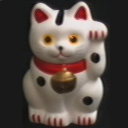
\includegraphics[width=0.1\textwidth,height=0.1\textwidth]{imagens/coil_100/animais_brinquedos/obj14__0.png} &
    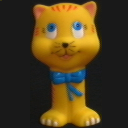
\includegraphics[width=0.1\textwidth,height=0.1\textwidth]{imagens/coil_100/animais_brinquedos/obj17__0.png} &
    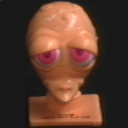
\includegraphics[width=0.1\textwidth,height=0.1\textwidth]{imagens/coil_100/animais_brinquedos/obj20__0.png} &
    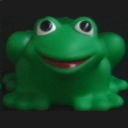
\includegraphics[width=0.1\textwidth,height=0.1\textwidth]{imagens/coil_100/animais_brinquedos/obj28__275.png} &
    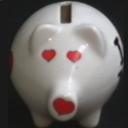
\includegraphics[width=0.1\linewidth,height=0.1\linewidth]{imagens/coil_100/animais_brinquedos/obj48__265.png} &
    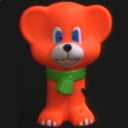
\includegraphics[width=0.1\linewidth,height=0.1\linewidth]{imagens/coil_100/animais_brinquedos/obj52__0.png} &
    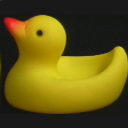
\includegraphics[width=0.1\linewidth,height=0.1\linewidth]{imagens/coil_100/animais_brinquedos/obj74__0.png}
    \\
    \scriptsize{obj01.jpg} & \scriptsize{obj02.jpg} & \scriptsize{obj03.jpg} &
    \scriptsize{obj04.jpg} & \scriptsize{obj05.jpg} & \scriptsize{obj06.jpg} &
    \scriptsize{obj07.jpg}
  \end{tabu}
\end{table}

\begin{table}[H]
  \centering
  \caption{Grupo B (barquinhos de brinquedo).}
  \tabulinesep =_0.5em^0.5em
  \everyrow{\tabucline[0.4pt]-}
  \begin{tabu}{|cccc|}
    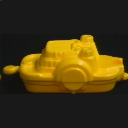
\includegraphics[width=0.1\textwidth,height=0.1\textwidth]{imagens/coil_100/barquinhos_brinquedos/obj3__0.png} &
    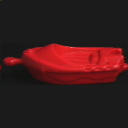
\includegraphics[width=0.1\textwidth,height=0.1\textwidth]{imagens/coil_100/barquinhos_brinquedos/obj38__0.png} &
    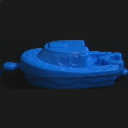
\includegraphics[width=0.1\textwidth,height=0.1\textwidth]{imagens/coil_100/barquinhos_brinquedos/obj42__0.png} &
    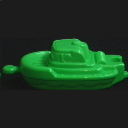
\includegraphics[width=0.1\textwidth,height=0.1\textwidth]{imagens/coil_100/barquinhos_brinquedos/obj78__0.png}
    \\
    \scriptsize{obj08.jpg} & \scriptsize{obj09.jpg} & \scriptsize{obj10.jpg} &
    \scriptsize{obj11.jpg}
  \end{tabu}
\end{table}

\begin{table}[H]
  \centering
  \caption{Grupo C (boias).}
  \tabulinesep =_0.5em^0.5em
  \everyrow{\tabucline[0.4pt]-}
  \begin{tabu}{|cc|}
    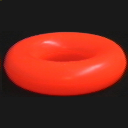
\includegraphics[width=0.1\textwidth,height=0.1\textwidth]{imagens/coil_100/boias/obj47__0.png} &
    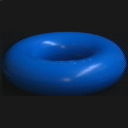
\includegraphics[width=0.1\textwidth,height=0.1\textwidth]{imagens/coil_100/boias/obj94__0.png}
    \\
    \scriptsize{obj12.jpg} & \scriptsize{obj13.jpg}
  \end{tabu}
\end{table}

\begin{table}[H]
  \centering
  \caption{Grupo D (caixas).}
  \tabulinesep =_0.5em^0.5em
  \everyrow{\tabucline[0.4pt]-}
  \begin{tabu}{|ccccc|}
    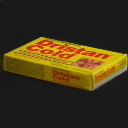
\includegraphics[width=0.1\textwidth,height=0.1\textwidth]{imagens/coil_100/caixas/obj1__35.png} &
    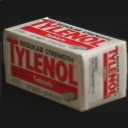
\includegraphics[width=0.1\textwidth,height=0.1\textwidth]{imagens/coil_100/caixas/obj31__45.png} &
    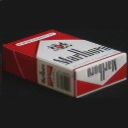
\includegraphics[width=0.1\textwidth,height=0.1\textwidth]{imagens/coil_100/caixas/obj46__45.png} &
    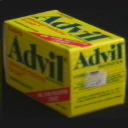
\includegraphics[width=0.1\textwidth,height=0.1\textwidth]{imagens/coil_100/caixas/obj54__55.png} &
    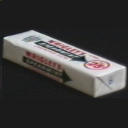
\includegraphics[width=0.1\textwidth,height=0.1\textwidth]{imagens/coil_100/caixas/obj67__50.png}
    \\
    \scriptsize{obj14.jpg} & \scriptsize{obj15.jpg} & \scriptsize{obj16.jpg} &
    \scriptsize{obj17.jpg} & \scriptsize{obj18.jpg}
    \\
    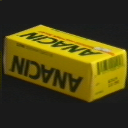
\includegraphics[width=0.1\textwidth,height=0.1\textwidth]{imagens/coil_100/caixas/obj79__45.png} &
    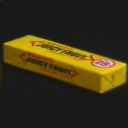
\includegraphics[width=0.1\textwidth,height=0.1\textwidth]{imagens/coil_100/caixas/obj84__45.png} &
    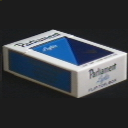
\includegraphics[width=0.1\textwidth,height=0.1\textwidth]{imagens/coil_100/caixas/obj96__45.png} &
    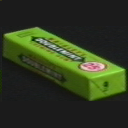
\includegraphics[width=0.1\textwidth,height=0.1\textwidth]{imagens/coil_100/caixas/obj98__55.png} &
    \\
    \scriptsize{obj19.jpg} & \scriptsize{obj20.jpg} & \scriptsize{obj21.jpg} &
    \scriptsize{obj22.jpg} &
  \end{tabu}
\end{table}

\begin{table}[H]
  \centering
  \caption{Grupo E (carrinhos de brinquedo).}
  \tabulinesep =_0.5em^0.5em
  \everyrow{\tabucline[0.4pt]-}
  \begin{tabu}{|cccccc|}
    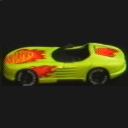
\includegraphics[width=0.1\textwidth,height=0.1\textwidth]{imagens/coil_100/carrinhos_brinquedos/obj6__0.png} &
    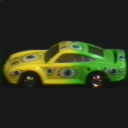
\includegraphics[width=0.1\textwidth,height=0.1\textwidth]{imagens/coil_100/carrinhos_brinquedos/obj8__0.png} &
    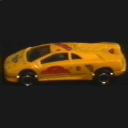
\includegraphics[width=0.1\textwidth,height=0.1\textwidth]{imagens/coil_100/carrinhos_brinquedos/obj15__0.png} &
    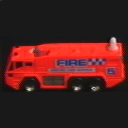
\includegraphics[width=0.1\textwidth,height=0.1\textwidth]{imagens/coil_100/carrinhos_brinquedos/obj19__0.png} &
    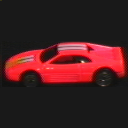
\includegraphics[width=0.1\textwidth,height=0.1\textwidth]{imagens/coil_100/carrinhos_brinquedos/obj23__0.png} &
    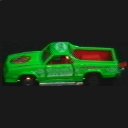
\includegraphics[width=0.1\textwidth,height=0.1\textwidth]{imagens/coil_100/carrinhos_brinquedos/obj27__0.png}
    \\
    \scriptsize{obj23.jpg} & \scriptsize{obj24.jpg} & \scriptsize{obj25.jpg} &
    \scriptsize{obj26.jpg} & \scriptsize{obj27.jpg} & \scriptsize{28obj.jpg}
    \\
    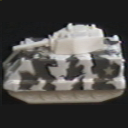
\includegraphics[width=0.1\textwidth,height=0.1\textwidth]{imagens/coil_100/carrinhos_brinquedos/obj37__0.png} &
    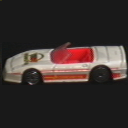
\includegraphics[width=0.1\textwidth,height=0.1\textwidth]{imagens/coil_100/carrinhos_brinquedos/obj69__0.png} &
    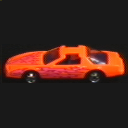
\includegraphics[width=0.1\textwidth,height=0.1\textwidth]{imagens/coil_100/carrinhos_brinquedos/obj76__0.png} &
    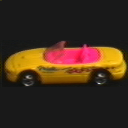
\includegraphics[width=0.1\textwidth,height=0.1\textwidth]{imagens/coil_100/carrinhos_brinquedos/obj91__0.png} &
    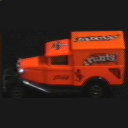
\includegraphics[width=0.1\textwidth,height=0.1\textwidth]{imagens/coil_100/carrinhos_brinquedos/obj100__0.png} &
    \\
    \scriptsize{obj29.jpg} & \scriptsize{obj30.jpg} & \scriptsize{obj31.jpg} &
    \scriptsize{obj32.jpg} & \scriptsize{obj33.jpg} &
  \end{tabu}
\end{table}

\begin{table}[H]
  \centering
  \caption{Grupo F (chícaras).}
  \tabulinesep =_0.5em^0.5em
  \everyrow{\tabucline[0.4pt]-}
  \begin{tabu}{|ccccc|}
    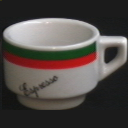
\includegraphics[width=0.1\textwidth,height=0.1\textwidth]{imagens/coil_100/chicaras/obj10__0.png} &
    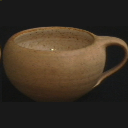
\includegraphics[width=0.1\textwidth,height=0.1\textwidth]{imagens/coil_100/chicaras/obj11__0.png} &
    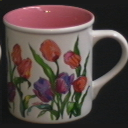
\includegraphics[width=0.1\textwidth,height=0.1\textwidth]{imagens/coil_100/chicaras/obj16__0.png} &
    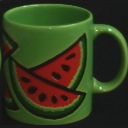
\includegraphics[width=0.1\textwidth,height=0.1\textwidth]{imagens/coil_100/chicaras/obj43__0.png} &
    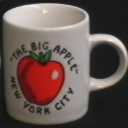
\includegraphics[width=0.1\textwidth,height=0.1\textwidth]{imagens/coil_100/chicaras/obj45__0.png}
    \\
    \scriptsize{obj34.jpg} & \scriptsize{obj35.jpg} & \scriptsize{obj36.jpg} &
    \scriptsize{obj37.jpg} & \scriptsize{obj38.jpg}
    \\
    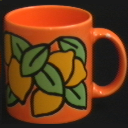
\includegraphics[width=0.1\textwidth,height=0.1\textwidth]{imagens/coil_100/chicaras/obj59__0.png} &
    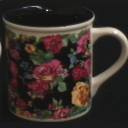
\includegraphics[width=0.1\textwidth,height=0.1\textwidth]{imagens/coil_100/chicaras/obj81__0.png} &
    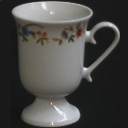
\includegraphics[width=0.1\textwidth,height=0.1\textwidth]{imagens/coil_100/chicaras/obj89__0.png} &
    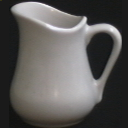
\includegraphics[width=0.1\textwidth,height=0.1\textwidth]{imagens/coil_100/chicaras/obj97__0.png} &
    \\
    \scriptsize{obj39.jpg} & \scriptsize{obj40.jpg} & \scriptsize{obj41.jpg} &
    \scriptsize{obj42.jpg} &
  \end{tabu}
\end{table}

\begin{table}[H]
  \centering
  \caption{Grupo G (embalagens cilíndricas).}
  \tabulinesep =_0.5em^0.5em
  \everyrow{\tabucline[0.4pt]-}
  \begin{tabu}{|ccccc|}
    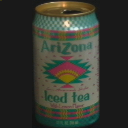
\includegraphics[width=0.1\textwidth,height=0.1\textwidth]{imagens/coil_100/embalagens_cilindricas/obj7__0.png} &
    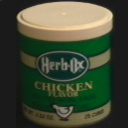
\includegraphics[width=0.1\textwidth,height=0.1\textwidth]{imagens/coil_100/embalagens_cilindricas/obj26__0.png} &
    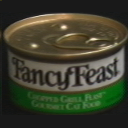
\includegraphics[width=0.1\textwidth,height=0.1\textwidth]{imagens/coil_100/embalagens_cilindricas/obj29__0.png} &
    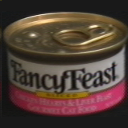
\includegraphics[width=0.1\textwidth,height=0.1\textwidth]{imagens/coil_100/embalagens_cilindricas/obj32__0.png} &
    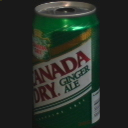
\includegraphics[width=0.1\textwidth,height=0.1\textwidth]{imagens/coil_100/embalagens_cilindricas/obj49__0.png}
    \\
    \scriptsize{obj43.jpg} & \scriptsize{obj44.jpg} & \scriptsize{obj45.jpg} &
    \scriptsize{obj46.jpg} & \scriptsize{obj47.jpg}
    \\
    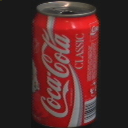
\includegraphics[width=0.1\textwidth,height=0.1\textwidth]{imagens/coil_100/embalagens_cilindricas/obj62__80.png} &
    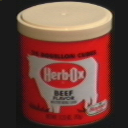
\includegraphics[width=0.1\textwidth,height=0.1\textwidth]{imagens/coil_100/embalagens_cilindricas/obj71__0.png} &
    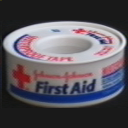
\includegraphics[width=0.1\textwidth,height=0.1\textwidth]{imagens/coil_100/embalagens_cilindricas/obj87__0.png} &
    \includegraphics[width=0.1\textwidth,height=0.1\textwidth]{imagens/coil_100/embalagens_cilindricas/obj93__0.png} &
    \includegraphics[width=0.1\textwidth,height=0.1\textwidth]{imagens/coil_100/embalagens_cilindricas/obj99__0.png}
    \\
    \scriptsize{obj48.jpg} & \scriptsize{obj49.jpg} & \scriptsize{obj50.jpg} &
    \scriptsize{obj51.jpg} & \scriptsize{obj52.jpg}
  \end{tabu}
\end{table}

\begin{table}[H]
  \centering
  \caption{Grupo H (embalagens retangulares).}
  \tabulinesep =_0.5em^0.5em
  \everyrow{\tabucline[0.4pt]-}
  \begin{tabu}{|cccccc|}
    \includegraphics[width=0.1\textwidth,height=0.1\textwidth]{imagens/coil_100/embalagens_retangulares/obj9__30.png} &
    \includegraphics[width=0.1\textwidth,height=0.1\textwidth]{imagens/coil_100/embalagens_retangulares/obj22__0.png} &
    \includegraphics[width=0.1\textwidth,height=0.1\textwidth]{imagens/coil_100/embalagens_retangulares/obj39__55.png} &
    \includegraphics[width=0.1\textwidth,height=0.1\textwidth]{imagens/coil_100/embalagens_retangulares/obj55__0.png} &
    \includegraphics[width=0.1\textwidth,height=0.1\textwidth]{imagens/coil_100/embalagens_retangulares/obj65__50.png} &
    \includegraphics[width=0.1\textwidth,height=0.1\textwidth]{imagens/coil_100/embalagens_retangulares/obj90__0.png}
    \\
    \scriptsize{obj53.jpg} & \scriptsize{obj54.jpg} & \scriptsize{obj55.jpg} &
    \scriptsize{obj56.jpg} & \scriptsize{obj57.jpg} & \scriptsize{obj58.jpg}
  \end{tabu}
\end{table}

\begin{table}[H]
  \centering
  \caption{Grupo I (embalagens com tampa).}
  \tabulinesep =_0.5em^0.5em
  \everyrow{\tabucline[0.4pt]-}
  \begin{tabu}{|ccccc|}
    \includegraphics[width=0.1\textwidth,height=0.1\textwidth]{imagens/coil_100/embalagens_tampas/obj5__0.png} &
    \includegraphics[width=0.1\textwidth,height=0.1\textwidth]{imagens/coil_100/embalagens_tampas/obj13__40.png} &
    \includegraphics[width=0.1\textwidth,height=0.1\textwidth]{imagens/coil_100/embalagens_tampas/obj24__0.png} &
    \includegraphics[width=0.1\textwidth,height=0.1\textwidth]{imagens/coil_100/embalagens_tampas/obj33__0.png} &
    \includegraphics[width=0.1\textwidth,height=0.1\textwidth]{imagens/coil_100/embalagens_tampas/obj50__0.png}
    \\
    \scriptsize{obj59.jpg} & \scriptsize{obj60.jpg} & \scriptsize{obj61.jpg} &
    \scriptsize{obj62.jpg} & \scriptsize{obj63.jpg}
    \\
    \includegraphics[width=0.1\textwidth,height=0.1\textwidth]{imagens/coil_100/embalagens_tampas/obj61__0.png} &
    \includegraphics[width=0.1\textwidth,height=0.1\textwidth]{imagens/coil_100/embalagens_tampas/obj64__0.png} &
    \includegraphics[width=0.1\textwidth,height=0.1\textwidth]{imagens/coil_100/embalagens_tampas/obj88__0.png} &
    \includegraphics[width=0.1\textwidth,height=0.1\textwidth]{imagens/coil_100/embalagens_tampas/obj92__0.png} &
    \\
    \scriptsize{obj64.jpg} & \scriptsize{obj65.jpg} & \scriptsize{obj66.jpg} &
    \scriptsize{obj67.jpg} &
  \end{tabu}
\end{table}

\begin{table}[H]
  \centering
  \caption{Grupo J (ganchos).}
  \tabulinesep =_0.5em^0.5em
  \everyrow{\tabucline[0.4pt]-}
  \begin{tabu}{|cc|}
    \includegraphics[width=0.1\textwidth,height=0.1\textwidth]{imagens/coil_100/ganchos/obj36__0.png} &
    \includegraphics[width=0.1\textwidth,height=0.1\textwidth]{imagens/coil_100/ganchos/obj85__0.png}
    \\
    \scriptsize{obj68.jpg} & \scriptsize{obj69.jpg}
  \end{tabu}
\end{table}

\begin{table}[H]
  \centering
  \caption{Grupo L (lanches).}
  \tabulinesep =_0.5em^0.5em
  \everyrow{\tabucline[0.4pt]-}
  \begin{tabu}{|cc|}
    \includegraphics[width=0.1\textwidth,height=0.1\textwidth]{imagens/coil_100/lanches/obj53__0.png} &
    \includegraphics[width=0.1\textwidth,height=0.1\textwidth]{imagens/coil_100/lanches/obj73__0.png}
    \\
    \scriptsize{obj70.jpg} & \scriptsize{obj71.jpg}
  \end{tabu}
\end{table}

\begin{table}[H]
  \centering
  \caption{Grupo M (legumes e frutas).}
  \tabulinesep =_0.5em^0.5em
  \everyrow{\tabucline[0.4pt]-}
  \begin{tabu}{|ccccccc|}
    \includegraphics[width=0.1\textwidth,height=0.1\textwidth]{imagens/coil_100/legumes_frutas/obj2__0.png} &
    \includegraphics[width=0.1\textwidth,height=0.1\textwidth]{imagens/coil_100/legumes_frutas/obj4__0.png} &
    \includegraphics[width=0.1\textwidth,height=0.1\textwidth]{imagens/coil_100/legumes_frutas/obj63__0.png} &
    \includegraphics[width=0.1\textwidth,height=0.1\textwidth]{imagens/coil_100/legumes_frutas/obj75__0.png} &
    \includegraphics[width=0.1\linewidth,height=0.1\linewidth]{imagens/coil_100/legumes_frutas/obj82__0.png} &
    \includegraphics[width=0.1\linewidth,height=0.1\linewidth]{imagens/coil_100/legumes_frutas/obj83__0.png} &
    \includegraphics[width=0.1\linewidth,height=0.1\linewidth]{imagens/coil_100/legumes_frutas/obj86__0.png}
    \\
    \scriptsize{obj72.jpg} & \scriptsize{obj73.jpg} & \scriptsize{obj74.jpg} &
    \scriptsize{obj75.jpg} & \scriptsize{obj76.jpg} & \scriptsize{obj77.jpg} &
    \scriptsize{obj78.jpg}
  \end{tabu}
\end{table}

\begin{table}[H]
  \centering
  \caption{Grupo N (objetos de madeira).}
  \tabulinesep =_0.5em^0.5em
  \everyrow{\tabucline[0.4pt]-}
  \begin{tabu}{|ccccc|}
    \includegraphics[width=0.1\textwidth,height=0.1\textwidth]{imagens/coil_100/objetos_madeira/obj12__0.png} &
    \includegraphics[width=0.1\textwidth,height=0.1\textwidth]{imagens/coil_100/objetos_madeira/obj41__0.png} &
    \includegraphics[width=0.1\textwidth,height=0.1\textwidth]{imagens/coil_100/objetos_madeira/obj51__0.png} &
    \includegraphics[width=0.1\textwidth,height=0.1\textwidth]{imagens/coil_100/objetos_madeira/obj77__0.png} &
    \includegraphics[width=0.1\linewidth,height=0.1\linewidth]{imagens/coil_100/objetos_madeira/obj80__0.png}
    \\
    \scriptsize{obj79.jpg} & \scriptsize{obj80.jpg} & \scriptsize{obj81.jpg} &
    \scriptsize{obj82.jpg} & \scriptsize{obj83.jpg}
  \end{tabu}
\end{table}

\begin{table}[H]
  \centering
  \caption{Grupo O (potes).}
  \tabulinesep =_0.5em^0.5em
  \everyrow{\tabucline[0.4pt]-}
  \begin{tabu}{|ccc|}
    \includegraphics[width=0.1\textwidth,height=0.1\textwidth]{imagens/coil_100/potes/obj70__0.png} &
    \includegraphics[width=0.1\textwidth,height=0.1\textwidth]{imagens/coil_100/potes/obj72__0.png} &
    \includegraphics[width=0.1\textwidth,height=0.1\textwidth]{imagens/coil_100/potes/obj95__0.png}
    \\
    \scriptsize{obj84.jpg} & \scriptsize{obj85.jpg} & \scriptsize{obj86.jpg}
  \end{tabu}
\end{table}

\begin{table}[H]
  \centering
  \caption{Grupo P (vasos).}
  \tabulinesep =_0.5em^0.5em
  \everyrow{\tabucline[0.4pt]-}
  \begin{tabu}{|ccccc|}
    \includegraphics[width=0.1\textwidth,height=0.1\textwidth]{imagens/coil_100/vasos/obj18__0.png} &
    \includegraphics[width=0.1\textwidth,height=0.1\textwidth]{imagens/coil_100/vasos/obj25__0.png} &
    \includegraphics[width=0.1\textwidth,height=0.1\textwidth]{imagens/coil_100/vasos/obj30__0.png} &
    \includegraphics[width=0.1\textwidth,height=0.1\textwidth]{imagens/coil_100/vasos/obj56__0.png} &
    \includegraphics[width=0.1\textwidth,height=0.1\textwidth]{imagens/coil_100/vasos/obj58__0.png}
    \\
    \scriptsize{obj87.jpg} & \scriptsize{obj88.jpg} & \scriptsize{obj89.jpg} &
    \scriptsize{obj90.jpg} & \scriptsize{obj91.jpg}
  \end{tabu}
\end{table}

\section{Considerações sobre a implementação e a plataforma de execução}

TEXTO AQUI.

\section{Treinamento da rede e convergência do erro}

TEXTO AQUI.

\section{Tempo de execução}

TEXTO AQUI.

\section{Disposição das imagens no mapa}

TEXTO AQUI.

\section{Variação da U-matriz e rotulação das imagens}

TEXTO AQUI.

\section{Avaliação geral dos resultados}

TEXTO AQUI.
